% Préambule commun aux manuels de Calque (français et anglais).
% Compilation : pdflatex manuel-fr.tex (deux fois), idem manuel-en.tex, depuis docs/src/.
\documentclass[11pt,a4paper]{article}
\usepackage[utf8]{inputenc}
\usepackage[T1]{fontenc}
\usepackage{lmodern}
\usepackage{microtype}
\usepackage[a4paper,margin=2cm,headheight=24pt]{geometry}
\usepackage{graphicx}
\usepackage[table]{xcolor}
\usepackage[most]{tcolorbox}
\usepackage{enumitem}
\usepackage{booktabs}
\usepackage{array}
\usepackage{tabularx}
\usepackage[nobottomtitles*]{titlesec}
\usepackage{needspace}
\usepackage{fancyhdr}
\usepackage{fontawesome5}
\usepackage{etoolbox}
\DeclareUnicodeCharacter{2192}{\ensuremath{\rightarrow}}
\DeclareUnicodeCharacter{2191}{\ensuremath{\uparrow}}
\DeclareUnicodeCharacter{2193}{\ensuremath{\downarrow}}
\DeclareUnicodeCharacter{25B2}{\ensuremath{\blacktriangle}}
\DeclareUnicodeCharacter{25BC}{\ensuremath{\blacktriangledown}}
\DeclareUnicodeCharacter{21BA}{\ensuremath{\circlearrowleft}}
\DeclareUnicodeCharacter{21BB}{\ensuremath{\circlearrowright}}
\usepackage{amssymb}

% Palette de l'application : papier calque, bleu de Prusse, ocre
\definecolor{bordeaux}{HTML}{1D4E73}
\definecolor{bordeauxl}{HTML}{E5EEF5}
\definecolor{or}{HTML}{C07A1E}
\definecolor{orl}{HTML}{FBF1E2}
\definecolor{sapin}{HTML}{2C7A55}
\definecolor{sapinl}{HTML}{E2F1E9}
\definecolor{sky}{HTML}{1C6DB4}
\definecolor{skyl}{HTML}{E6F0F8}
\definecolor{summit}{HTML}{6B7A8F}
\definecolor{night}{HTML}{1F2A33}
\definecolor{ink}{HTML}{1F2430}
\AtBeginDocument{\color{ink}}

\titleformat{\section}
  {\Large\bfseries\sffamily\color{bordeaux}}
  {\makebox[1.6em][l]{\thesection}}{0.3em}{}
  [{\vspace{1pt}\color{bordeaux!35}\titlerule[1.3pt]}]
\titlespacing*{\section}{0pt}{14pt}{7pt}
\titleformat{\subsection}{\large\bfseries\sffamily\color{night}}{\thesubsection}{0.5em}{}
\pretocmd{\section}{\needspace{10\baselineskip}}{}{}
\pretocmd{\subsection}{\needspace{7\baselineskip}}{}{}
\widowpenalty=10000
\clubpenalty=10000
\raggedbottom
\setlength{\parindent}{0pt}
\setlength{\parskip}{6pt}
\setlist[enumerate]{itemsep=3pt,leftmargin=6mm}
\setlist[itemize]{itemsep=2pt,leftmargin=5mm}

\pagestyle{fancy}
\fancyhf{}
\renewcommand{\headrulewidth}{0.4pt}
\renewcommand{\headrule}{\hbox to\headwidth{\color{bordeaux!40}\leaders\hrule height \headrulewidth\hfill}}
\fancyfoot[C]{\sffamily\small\color{summit}\thepage}
\renewcommand{\sectionmark}[1]{\markboth{#1}{}}

\newcommand{\menu}[1]{\textsf{\textbf{\textcolor{bordeaux}{#1}}}}
\newcommand{\touche}[1]{\tcbox[on line,boxsep=0pt,left=2pt,right=2pt,top=1.5pt,bottom=1.5pt,
  colback=white,colframe=summit,boxrule=0.5pt,arc=1.5pt]{\footnotesize\textsf{#1}}}
\newcommand{\fichier}[1]{\texttt{\small #1}}

\newcommand{\boite}[5]{\newtcolorbox{#1}{enhanced,unbreakable,colback=#2,colframe=#3,
  coltitle=white,fonttitle=\bfseries\sffamily\small,boxrule=0.9pt,arc=2.5pt,
  left=2.5mm,right=2.5mm,top=1.2mm,bottom=1.2mm,title={#4~~#5}}}
\newcommand{\capture}[2][1]{\par\needspace{8\baselineskip}\begin{center}\setlength{\fboxsep}{0pt}\setlength{\fboxrule}{0.6pt}%
  \fcolorbox{summit!50}{white}{\includegraphics[width=\dimexpr#1\linewidth-1.3pt\relax]{#2}}\end{center}}

\definecolor{rouge}{HTML}{A33A2E}
\definecolor{rougel}{HTML}{F8E6E3}

\usepackage[french]{babel}
\usepackage[colorlinks=true,linkcolor=bordeaux,urlcolor=bordeaux]{hyperref}
\hypersetup{pdftitle={Calque — manuel d'utilisation},pdfauthor={},pdfcreator={Calque}}
\boite{astucebox}{orl}{or!85!black}{\faLightbulb}{Bon à savoir}
\boite{securitebox}{sapinl}{sapin}{\faShield*}{Votre disque actuel est protégé}
\boite{attentionbox}{rougel}{rouge}{\faExclamationTriangle}{Attention}
\newcommand{\astuce}[1]{\par\needspace{5\baselineskip}\begin{astucebox}#1\end{astucebox}}
\newcommand{\attention}[1]{\par\needspace{5\baselineskip}\begin{attentionbox}#1\end{attentionbox}}
\fancyhead[L]{\sffamily\small\color{bordeaux}\textbf{CALQUE — MANUEL}}
\fancyhead[R]{\sffamily\small\color{summit}\leftmark}
\input{version}

\begin{document}

\begin{titlepage}
\centering
\vspace*{2.2cm}
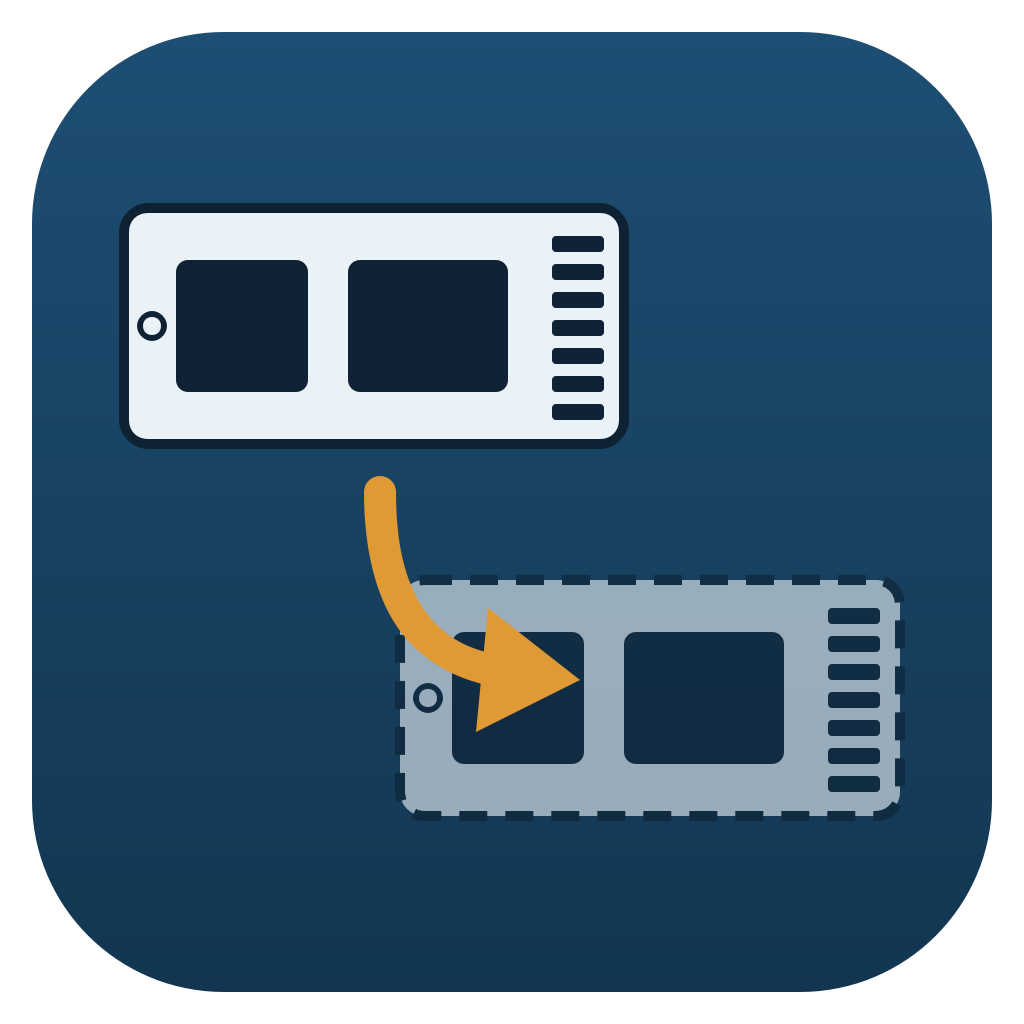
\includegraphics[width=3.6cm]{../../logo_1024.png}\par
\vspace{8mm}
{\sffamily\Huge\bfseries\color{bordeaux} CALQUE\par}
\vspace{3mm}
{\sffamily\LARGE\color{ink} Cloner un disque — Windows compris —\\ sur un disque plus grand\par}
\vspace{2mm}
{\sffamily\large\color{summit} Manuel d'utilisation \textbullet{} version \versioncalque\par}
\vspace{12mm}
\begin{tcolorbox}[enhanced,width=0.82\linewidth,colback=orl,colframe=or,arc=4pt,boxrule=1.2pt,left=5mm,right=5mm,top=3mm,bottom=3mm]
\sffamily\centering
\textit{Calque} : la copie fidèle d'un dessin, trait pour trait.\\[2mm]
\raggedright
Trois gestes :\\[1mm]
\textbf{choisir les deux disques} \quad → \quad \textbf{lire le plan} \quad → \quad \textbf{Cloner}\\[1mm]
puis, une fois le nouveau disque en place : \textbf{Agrandir C:}.
\end{tcolorbox}
\vfill
{\footnotesize\color{summit}\sffamily Windows (à chaud) \textbullet{} Linux (depuis une clé USB)\par}
\end{titlepage}

\tableofcontents
\newpage

\section{À quoi sert Calque}

Votre disque système est trop petit, et vous avez acheté un disque plus grand. Calque recopie
\textbf{tout} l'ancien disque sur le nouveau — partitions cachées de Windows comprises — de sorte
que l'ordinateur redémarre sur le nouveau disque \textbf{exactement comme avant}, sans réinstaller
Windows ni vos logiciels. L'espace gagné est ensuite rendu à C: d'un clic.

\begin{securitebox}
\begin{itemize}
\item Le disque source n'est \textbf{jamais modifié} : Calque le lit, il n'écrit que sur la cible.
\item Le disque système en cours d'utilisation ne peut pas être choisi comme cible.
\item Avant d'effacer la cible, Calque montre ce qu'elle va devenir et demande deux confirmations.
\item Chaque bloc copié est \textbf{relu et comparé} : une liaison USB défaillante est détectée.
\item Une interruption (annulation, câble débranché, panne) laisse la cible \textbf{vide} : elle ne
      peut pas être prise pour un clone complet.
\end{itemize}
\end{securitebox}

\section{Avant de commencer}

\begin{enumerate}
\item \textbf{Sauvegardez vos documents importants} ailleurs (clé, disque externe, nuage). Calque ne
      touche pas à la source, mais une sauvegarde reste la règle avant toute opération sur un disque.
\item \textbf{BitLocker} : si C: est chiffré (fréquent sur les portables récents, « chiffrement de
      l'appareil »), déchiffrez-le d'abord (\menu{Paramètres → Confidentialité et sécurité →
      Chiffrement de l'appareil}, ou \texttt{manage-bde -off C:} dans un terminal administrateur) et
      attendez la fin. Calque le détecte et refuse sinon.
\item \textbf{Branchez le nouveau disque} : à l'intérieur du PC, ou dans un boîtier USB.
\item \textbf{Taille} : la cible doit être au moins aussi grande que la partie occupée par les
      partitions de la source (un 500~Go va sur un 500~Go ou plus ; Calque calcule et vous le dit).
\end{enumerate}

\attention{\textbf{Boîtiers USB et secteurs de 4096 octets.} Certains boîtiers (surtout pour disques
SATA de grande taille) présentent le disque à Windows avec des secteurs de 4096 octets au lieu de
512. Une copie écrite à travers un tel boîtier \textbf{ne démarre pas} une fois le disque monté dans
le PC : la table de partitions n'est plus lue au bon endroit. C'est une cause fréquente de clonages
« réussis » qui n'amorcent pas. Calque compare les deux disques et \textbf{refuse} dans ce cas, en
l'expliquant (figure~\ref{fig:4k}). Solution : un autre boîtier, le disque branché à l'intérieur, ou le
clonage sous Linux (section~\ref{sec:linux}).}

\section{Installer et lancer Calque}

\subsection*{Windows}
Téléchargez \fichier{Calque-Setup.exe} sur la page \textbf{Releases} du projet et lancez-le
(installation pour votre compte, sans droits particuliers). Calque demande ensuite, \textbf{à chaque
lancement}, les droits d'administrateur : lire et écrire un disque entier l'exige.

\subsection*{Linux}
Téléchargez \fichier{Calque-linux-x86\_64.tar.gz}, décompressez-le, lancez \fichier{installer.sh},
puis démarrez Calque \textbf{avec sudo} : \texttt{sudo \textasciitilde/.local/bin/calque}.
Si la fenêtre ne s'ouvre pas (session Wayland qui refuse les fenêtres de l'administrateur), tapez
d'abord \texttt{xhost +si:localuser:root}, ou utilisez la ligne de commande (dernière section).

\section{Cloner sous Windows, sans éteindre}\label{sec:windows}

Calque copie le disque \textbf{pendant que Windows tourne}. Pour que la copie soit cohérente, il
prend d'abord un \textbf{cliché instantané} (VSS) de chaque volume en service : une image figée de
C: à cet instant. Vous pouvez continuer à utiliser l'ordinateur ; simplement, ce que vous modifiez
pendant la copie ne sera pas sur le clone. Le plus simple : fermer ses documents et laisser faire.

\capture{../capture_plan-fr.png}

\begin{enumerate}
\item \textbf{Source} : Calque propose d'office le disque du système en cours.
\item \textbf{Cible} : le nouveau disque. Le disque système n'apparaît jamais dans cette liste. Après
      avoir branché un disque, cliquez sur \menu{Actualiser la liste}.
\item Lisez le \textbf{plan} : la barre « Aujourd'hui » montre la source, « Après » la cible, à la
      même échelle. Les petites partitions de Windows (EFI, réservée) sont au début ; C: garde sa
      place ; la partition de \textbf{récupération} est reportée en fin de disque, et la zone hachurée
      « libre » est l'espace gagné, juste derrière C:.
\item Laissez cochée la \textbf{relecture} (vérification). Elle double la durée mais prouve la copie.
\item Cochez la case « Je sais que TOUT le contenu… sera effacé », cliquez sur \menu{Cloner}, et
      confirmez une seconde fois.
\end{enumerate}

\capture{../capture_copie-fr.png}

Seuls les blocs \textbf{occupés} de C: sont copiés : un disque de 500~Go rempli à 150~Go ne copie
qu'environ 150~Go. Par USB 3, comptez 5 à 15~minutes par 100~Go, autant pour la vérification.

Le plan annonce aussi \textbf{combien de données seront copiées et une fourchette de durée}.
Pendant la copie, Calque \textbf{empêche Windows de se mettre en veille} (la veille couperait la
liaison USB).

\astuce{\menu{Annuler} arrête proprement : ce qui est copié est gardé, la cible n'a pas encore de
table de partitions (rien ne démarrera dessus par erreur) et le disque source n'a pas bougé. Le
bouton \menu{Reprendre} continue plus tard là où on s'est arrêté.}

\section{Si le boîtier USB décroche}\label{sec:decroche}

Les boîtiers USB pour SSD NVMe \textbf{chauffent} quand on y écrit des dizaines de Go d'affilée ;
certains se déconnectent alors quelques secondes, ou pour de bon. C'est la première cause de
clonage qui s'arrête en cours de route. Calque est fait pour ça :

\begin{itemize}
\item \textbf{Ménager le boîtier USB} (case cochée d'office quand la cible est en USB) : la copie est
      bridée à 200~Mo/s. C'est un peu plus long, mais le boîtier chauffe nettement moins.
\item \textbf{Décrochage bref} : Calque attend le retour du disque (jusqu'à 1~min~30), le retrouve
      même s'il a changé de numéro, et continue tout seul. Le message de fin dit combien de fois.
\item \textbf{Décrochage définitif} : Calque s'arrête proprement et garde ce qui est fait. Suivez le
      message : débranchez le boîtier, laissez-le refroidir une minute, rebranchez-le (port à
      l'arrière du PC, boîtier à plat, à l'air), \menu{Actualiser la liste}, puis \menu{Reprendre}.
\end{itemize}

\capture{../capture_reprise-fr.png}

Sous Windows, la reprise relit \textbf{le même cliché} qu'au début : le clone reste cohérent même si
vous avez travaillé entre-temps. Si le cliché a disparu (redémarrage du PC, nettoyage de disque),
Calque le dit et il faut recommencer de zéro.

\astuce{\textbf{Le plus fiable de tout} : pas d'USB du tout. Si votre carte mère n'a qu'un emplacement
M.2, une carte adaptateur PCIe → M.2 (une quinzaine d'euros) dans un emplacement PCIe libre permet de
mettre le nouveau SSD à l'intérieur, à côté de l'ancien, le temps du clonage.}

\section{Si le disque source a des zones illisibles}

Un disque qui vieillit peut avoir des secteurs qu'il n'arrive plus à lire. Calque réessaie plusieurs
fois, morceau par morceau, puis s'arrête et vous prévient : \textbf{votre disque actuel est peut-être
en train de s'abîmer}. Commencez par copier vos documents importants ailleurs.

Vous pouvez ensuite \menu{Continuer malgré tout} : les secteurs illisibles sont remplacés par des
zéros (le reste est copié normalement, et la copie reprend où elle s'était arrêtée). Le message de fin
indique leur nombre ; au premier démarrage sur le nouveau disque, lancez \texttt{chkdsk C: /f}.

\section{Cloner sous Linux, depuis une clé USB}\label{sec:linux}

C'est la méthode la plus sûre : Windows est \textbf{éteint}, son disque ne change pas pendant la
copie, aucun cliché n'est nécessaire. Elle est aussi la solution quand le boîtier USB pose problème,
puisqu'on peut monter le nouveau disque à l'intérieur du PC, à côté de l'ancien.

\begin{enumerate}
\item Préparez une clé USB « live » d'une distribution Linux (Ubuntu, Linux Mint, Fedora…).
\item Dans Windows, désactivez le \textbf{démarrage rapide} (\menu{Panneau de configuration →
      Options d'alimentation → Choisir l'action des boutons}), puis éteignez : sinon Windows laisse
      son disque dans un état « en veille prolongée ».
\item Démarrez sur la clé, sans installer Linux (« Essayer »).
\item Installez et lancez Calque avec \texttt{sudo} (section précédente), ou en ligne de commande :
      \texttt{sudo calque -{}-lister} puis \texttt{sudo calque -{}-cloner /dev/nvme0n1 /dev/sdb}.
\item Choisissez source et cible comme sous Windows. Calque refuse une source dont une partition
      est montée en écriture (sur une clé live, rien ne l'est par défaut).
\end{enumerate}

\section{Après le clonage}\label{sec:apres}

\begin{enumerate}
\item \textbf{Éteignez} l'ordinateur.
\item \textbf{Mettez le nouveau disque à la place de l'ancien} (ou débranchez l'ancien).
      Windows ne démarre pas depuis un boîtier USB : le disque doit être à l'intérieur.
\item \textbf{Démarrez.} Windows s'ouvre comme avant, sur le nouveau disque.
\item Lancez Calque, onglet \menu{Après le clonage}, et cliquez sur \menu{Agrandir C:}. C: prend
      tout l'espace libre, sans redémarrage, en quelques secondes.
\end{enumerate}

\capture{../capture_apres-fr.png}

\attention{\textbf{Ne démarrez pas avec les deux disques branchés} la première fois. Le clone porte
les mêmes identifiants que l'original (c'est ce qui lui permet de démarrer) : Windows pourrait
démarrer sur l'un et monter des partitions de l'autre. Il met d'ailleurs le second « hors ligne »
(« collision de signature »). Pour réutiliser l'ancien disque comme disque de données, branchez-le
\textbf{après}, et effacez-le dans \menu{Gestion des disques}.}

\subsection*{Environnement de récupération}
La partition de récupération a été déplacée en fin de disque. Si \texttt{reagentc /info} (terminal
administrateur) indique l'environnement de récupération « Disabled », ou si une mise à jour de
Windows s'en plaint, le bouton \menu{Réparer l'environnement de récupération} le désactive puis le
réactive, ce qui le réenregistre à sa nouvelle place.

\section{Quand ça ne marche pas}

\begin{center}
\renewcommand{\arraystretch}{1.35}
\begin{tabularx}{\linewidth}{>{\raggedright\arraybackslash}p{0.36\linewidth} >{\raggedright\arraybackslash}X}
\toprule
\textbf{Ce qu'on voit} & \textbf{Ce qu'il faut faire} \\
\midrule
« Secteurs de 512 octets sur la source, 4096 sur la cible » & Le boîtier USB pose le problème décrit
page~\pageref{fig:4k} : autre boîtier, disque à l'intérieur, ou Linux. \\
« La cible est trop petite » & Il faut une cible au moins aussi grande que l'indiqué. \\
« Un volume est chiffré par BitLocker » & Déchiffrer C: d'abord, attendre la fin, relancer. \\
« Disque dynamique ou Espaces de stockage » & Non pris en charge (rare sur un PC personnel). \\
« Accès refusé » & Lancer Calque en administrateur (Windows) ou avec \texttt{sudo} (Linux). \\
« La relecture a trouvé des blocs différents » & Câble, port ou boîtier USB défaillant, ou disque
cible abîmé : changer de câble ou de port (de préférence à l'arrière du PC) et recommencer. \\
« Le nouveau disque s'est déconnecté » & Voir section~\ref{sec:decroche} : refroidir, rebrancher,
\menu{Reprendre}. \\
« Zone illisible sur le disque source » & Sauvegarder ses documents, puis \menu{Continuer malgré
tout}. \\
Le PC ne démarre pas sur le nouveau disque & Dans le BIOS/UEFI, choisir le nouveau disque (entrée
« Windows Boot Manager ») comme premier périphérique de démarrage ; vérifier que l'ancien est bien
débranché. \\
\bottomrule
\end{tabularx}
\end{center}

\begin{figure}[h]
\capture{../capture_4k-fr.png}
\caption{Cible vue à travers un boîtier USB en secteurs de 4096 octets : clonage refusé.}\label{fig:4k}
\end{figure}

\section{Ce que fait Calque, exactement}

\begin{enumerate}
\item \textbf{Lecture} de la table de partitions de la source (GPT ou MBR), contrôlée par ses sommes de
      contrôle.
\item \textbf{Plan} : même disposition sur la cible ; les partitions situées après la plus grande
      (récupération) sont reportées en fin de disque, alignées sur 1~Mio.
\item \textbf{Clichés} des volumes en service (Windows), supprimés à la fin quoi qu'il arrive.
\item \textbf{Effacement} du début et de la fin de la cible (anciennes tables).
\item \textbf{Copie} partition par partition ; pour NTFS, seuls les blocs marqués occupés dans la carte
      d'allocation du volume ; chaque bloc reçoit une empreinte.
\item \textbf{Relecture} de la cible et comparaison des empreintes.
\item \textbf{Retouche} des secteurs d'amorçage des volumes déplacés (position de la partition).
\item \textbf{Table de partitions} écrite en dernier, avec les \textbf{mêmes identifiants} (GUID du
      disque et des partitions en GPT, signature en MBR) : le gestionnaire de démarrage de Windows
      désigne ses partitions par ces identifiants.
\end{enumerate}

\section{Ligne de commande}

\begin{tabular}{>{\ttfamily}l l}
calque -{}-lister & liste les disques (numéro, modèle, taille, secteurs) \\
calque -{}-cloner 0 2 & clone le disque 0 sur le disque 2 (Windows) \\
calque -{}-cloner /dev/nvme0n1 /dev/sdb & idem sous Linux \\
\quad -{}-oui & sans demander de confirmation \\
\quad -{}-sans-verification & sans relecture \\
\quad -{}-garder-place & sans déplacer la partition de récupération \\
\end{tabular}

\end{document}
